% !TeX spellcheck = en_GB
% %%% ***************** CHAPTER INSTRUMENTS, AND RETRIEVAL ***************** %%%
\chapter{Instruments and snowfall retrieval} \label{ch:DIM}
\textcolor{red}{\textbf{The overleaf file from the Methodology is here:} \\ \url{https://www.overleaf.com/13946091vphmgxbbxpyg}}

Many factors such as humidity and temperature contribute to snowflake geometry. The knowledge of snowflake habits, particle size distributions, and fall speed lead to a reduction of errors in optimal estimation retrievals. \\
This work is based on several datasets collected at the Haukeliseter measurement site, \ang{59.8}\,N, \ang{7.2}\,E. A composition of advanced ground based observations and the CloudSat precipitation retrieval will help to get a better understanding of the vertical structure of the atmosphere. 
\\
%%%%%%%%%%%%%%%%%%%%%%%%%%%%%%%%%%%%%%%%%%%%%%%%%%%%%%%%%%%%%%%%%%%%%%%%%%
%%%%%%%%%%%%%%%%%%%%%%%%%%%%%%%%%%%%%%%%%%%%%%%%%%%%%%%%%%%%%%%%%%%%%%%%%%
%%%%%%%%% INTSTRUMENTS %%%%%%%%%%%%%%
%\section{Instruments}\label{sec:instruments}
A collaboration between the University of Utah, University of Wisconsin and Met-Norway made it possible to install three additional instruments at the measurement site during winter 2016/2017. A Multi-Angle Snowflake Camera (MASC) and a Precipitation Imaging Package (PiP) will be used to determine the snow habit, the snowfall particle size distribution, and near-surface fall speed. Additionally, a Micro Rain Radar (MRR) is established to obtain fall speed and particle reflectivity aloft. Together with temperature observations at the surface, is this a good basis to reduce the non-uniquness of snow accumulation in optimal estimation snowfall retrieval, described in \Cref{sec:retrieval}. 
%
%
\pagebreak
%%%%%%%%%%%%%%%%%%%%%%%%%%%%%%%%%%%%%%%%%%%%%%%%%%%%%%%%%%%%%%%%%%%%%%%%%%
%%%%%%%%%%%%%%%%%%%%%%%%%%%%%%%%%%%%%%%%%%%%%%%%%%%%%%%%%%%%%%%%%%%%%%%%%%
%%%%%%%%% DOUBLE FENCE %%%%%%%%%%%%%%
\section{Double Fence}
%%% image double fence @ Haukeli %%%%%%%%%%%%%%%%%%%%%%%%%%%%%%%%%%%%%
% !TeX spellcheck = en_GB
% \begin{figure}[h!]
% 	\centering
% 		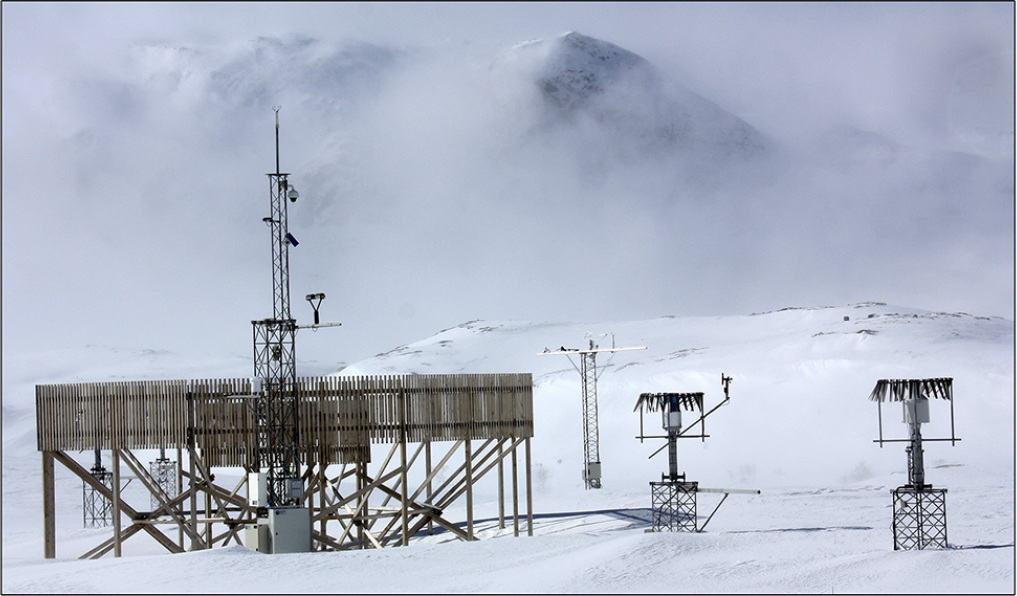
\includegraphics[width=0.55\textwidth]{./fig_instruments/Dofe.png}
% 	\caption{Picture, showing the double fence and unprotected precipitation gauges at the measurement site Haukeliseter. Picture taken from \cite{wolff_derivation_2015}.}\label{fig:Dofe}
% \end{figure}



\begin{wrapfigure}[28]{r}{0.44\textwidth}
	\vspace{-\normalbaselineskip}
	\centering
	\begin{subfigure}[b]{0.4\textwidth}
		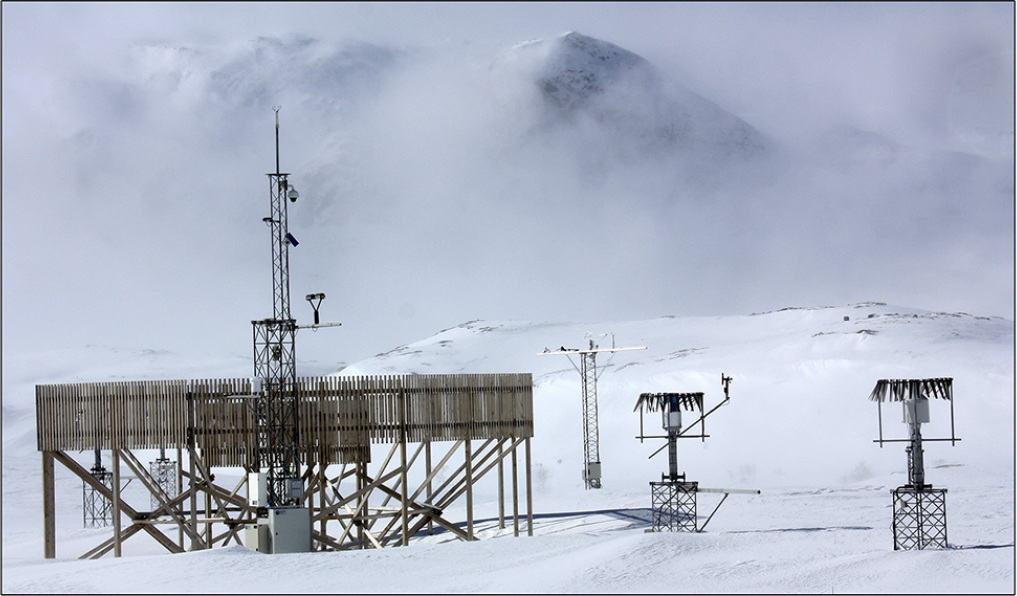
\includegraphics[width=\textwidth]{./fig_instruments/Dofe.png}
		\caption{}\label{fig:dofe_pic}
	\end{subfigure}	
	\begin{subfigure}[b]{0.4\textwidth}
		% 		\includegraphics[trim={0.8cm, 2.3cm, 2.4cm, 3cm},clip,width=1.1\textwidth]
		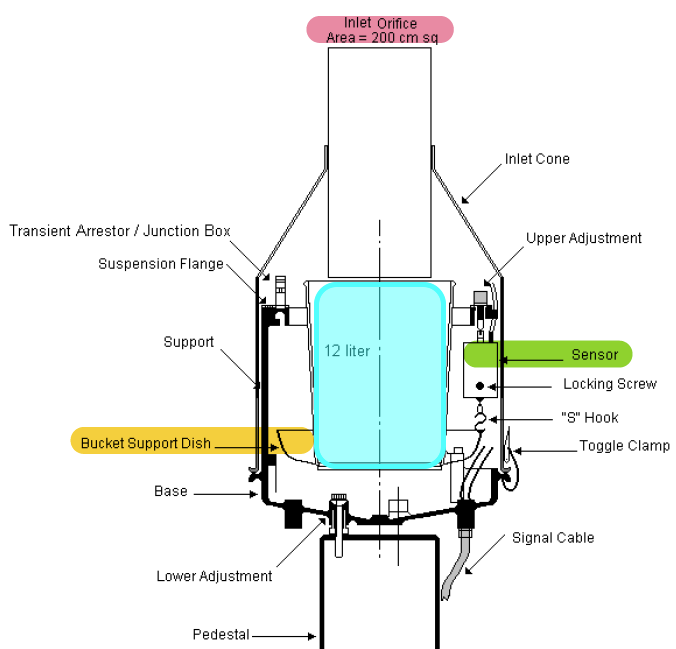
\includegraphics[width=1.1\textwidth]{./fig_instruments/Geonor_sketch2.png}
		\caption{}\label{fig:gauge_sketch}
	\end{subfigure}	
	\caption{(\protect\subref{fig:dofe_pic}) From left to right: Double fence gauge (\textbf{X0}) and unprotected precipitation gauges (\textbf{Nord, X4}) at Haukeliseter, from \cite{wolff_derivation_2015}. The prevailing easterly (westerly) wind from the lower, left corner in \protect\subref{fig:dofe_pic} (the opposite site). In front of the double fence gauge is the \SI{10}{\metre} weather mast (\textbf{M1}). (\protect\subref{fig:gauge_sketch}) Vertical cross section of Geonor T-200B3 precipitation gauge. pink: orifice; cyan: cylindric bucket with frost protection; yellow: bucket support dish; green: wire sensor \citep[adapted from][]{geonor_inc._t-200b_2015}.  }\label{fig:Dofe}
	%	\vspace{-\normalbaselineskip}
\end{wrapfigure}
%%%%%%%%%%%%%%%%%%%%%%%%%%%%%%%%%%%%%%%%%%%%%%%%%%%%%%%%%%%%%%%%%%%%%%%%%%
Since the winter season 2010/2011 Haukeliseter is equipped with three rain gauges. The wind shielded gauges are placed perpendicular to the main wind direction (\Cref{fig:Dofe}). The precipitation gauge protected by an octagonal double fence will be the reference to all surface accumulation measurements. The double fence creates an artificial calm wind and maximize the catch of precipitation, \citep{wolff_new_2010, wolff_measurements_2013, wolff_derivation_2015}. \textcolor{red}{This will get some more description. I have to read some up}
%%% image Dofe, MRR, MASC %%%%%%%%%%%%%%%%%%%%%%%%%%%%%%%%%%%%%
%% % !TeX spellcheck = en_GB
\begin{wrapfigure}{r}{0.44\textwidth}
	%	\vspace{-\normalbaselineskip}
	\centering
	\begin{subfigure}[b]{0.4\textwidth}
		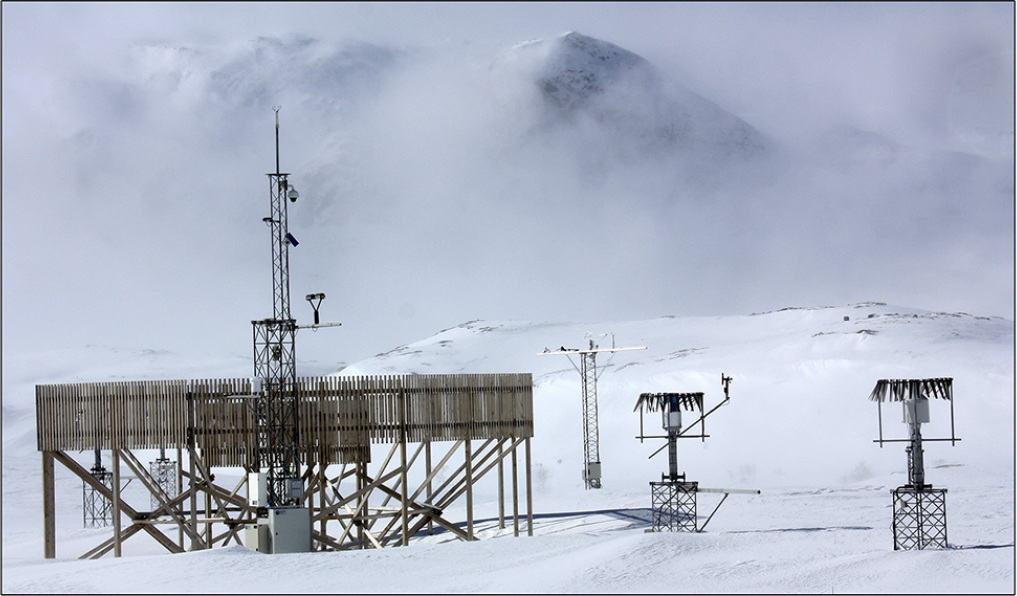
\includegraphics[width=\textwidth]{./fig_instruments/Dofe.png}
		\caption{}\label{fig:Dofe}
	\end{subfigure}
	\begin{subfigure}[b]{0.4\textwidth}
		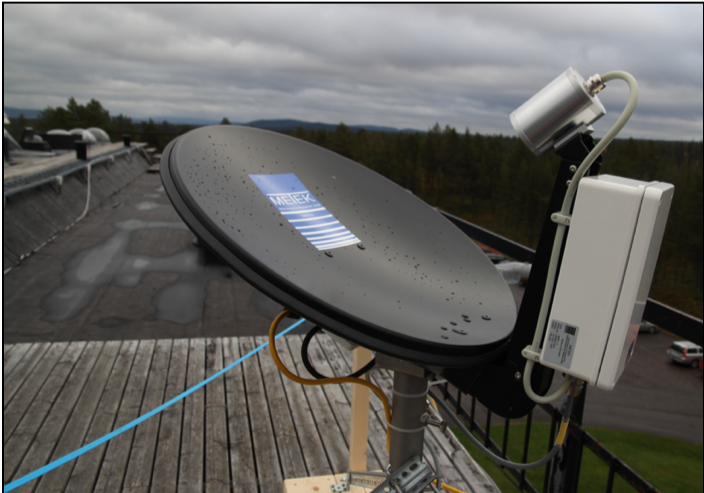
\includegraphics[width=\textwidth]{./fig_instruments/MRR.png}
		\caption{}\label{fig:MRR}
	\end{subfigure}
	\begin{subfigure}[b]{0.4\textwidth}
		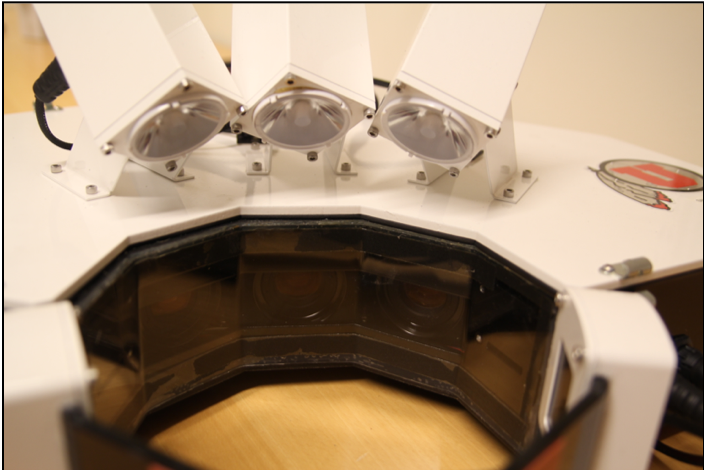
\includegraphics[width=\textwidth]{./fig_instruments/MASC.png}
	\end{subfigure}	
	\begin{subfigure}[b]{0.4\textwidth}
		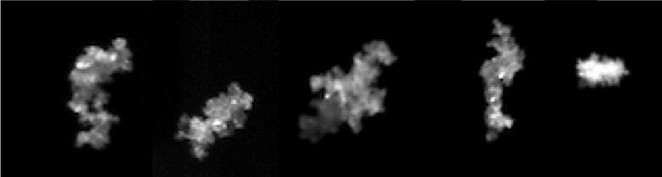
\includegraphics[width=\textwidth]{./fig_instruments/MASC_snowflakes.png}
		\caption{}\label{fig:MASC}
	\end{subfigure}	
	\caption{\protect\subref{fig:Dofe}: Double fence and unprotected precipitation gauges at Haukeliseter, from \cite{wolff_derivation_2015}. \protect\subref{fig:MRR}: Micro Rain Radar. \protect\subref{fig:MASC}: MASC and images taken by instrument. \textcolor{red}{Lower panel taken from \cite{cooper_variational_2017} maybe we get one for Haukeli?}}
	\vspace{-\normalbaselineskip}
\end{wrapfigure}

%%%%%%%%%%%%%%%%%%%%%%%%%%%%%%%%%%%%%%%%%%%%%%%%%%%%%%%%%%%%%%%%%%%%%%%%%%

%%%%%%%%%%%%%%%%%%%%%%%%%%%%%%%%%%%%%%%%%%%%%%%%%%%%%%%%%%%%%%%%%%%%%%%%%%
%%%%%%%%%%%%%%%%%%%%%%%%%%%%%%%%%%%%%%%%%%%%%%%%%%%%%%%%%%%%%%%%%%%%%%%%%%
%%%%%%%%% MRR %%%%%%%%%%%%%%
\section{MRR - Micro Rain Radar}
%%% image MRR instrument %%%%%%%%%%%%%%%%%%%%%%%%%%%%%%%%%%%%%
% !TeX spellcheck = en_GB
% \begin{figure}[h!]
% 	\centering
% 		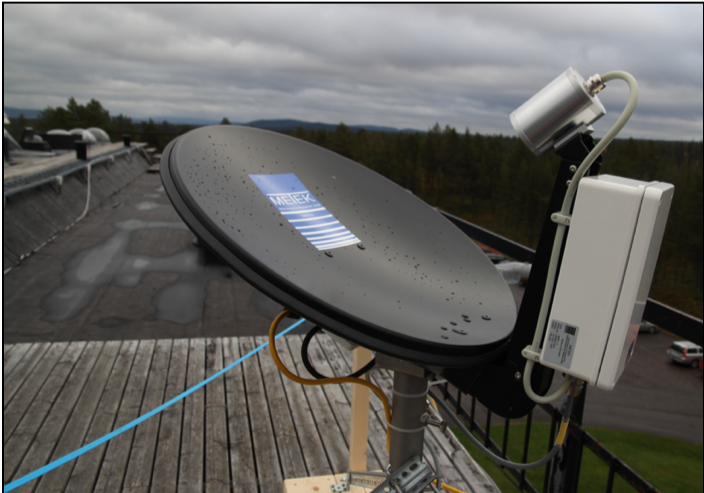
\includegraphics[width=0.55\textwidth]{./fig_instruments/MRR.png}
% 	\caption{MRR from METEK}\label{fig:MRR}
% \end{figure}

\begin{wrapfigure}[14]{r}{0.44\textwidth}
	\vspace{-\normalbaselineskip}
	\centering
	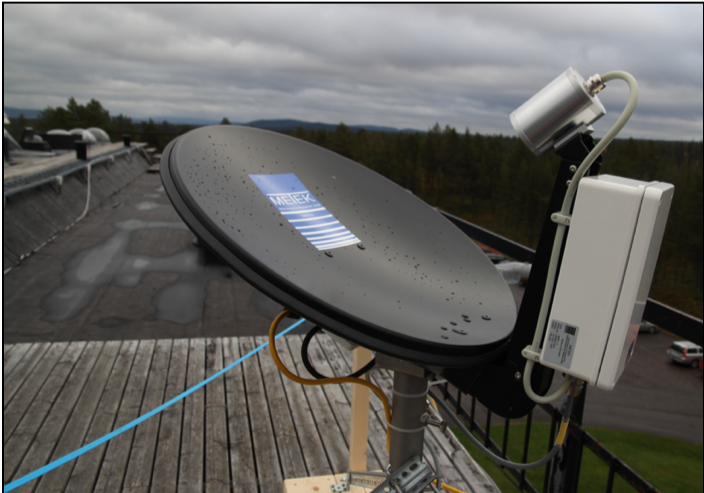
\includegraphics[width=0.4\textwidth]{./fig_instruments/MRR.png}
	%	\vspace{-10pt}
	\caption{Micro Rain Radar at the measurement site in Kiruna. Transceiver transmits Radar signal using the antenna (parabolic dish) and receives backscatter signal over the antenna. During winter 2016/2017 installed at Haukeliseter (\textbf{container}).}\label{fig:MRR}
	\vspace{-\normalbaselineskip}
\end{wrapfigure}
%%%%%%%%%%%%%%%%%%%%%%%%%%%%%%%%%%%%%%%%%%%%%%%%%%%%%%%%%%%%%%%%%%%%%%%%%%
Radars are very useful to observe the vertical of the atmosphere. The instrument is able to detect mesoscale features and makes it possible to see the vertical structure of storms \citep{markowski_mesoscale_2011}.\\
The principle of radar measurements is based on an electromagnetic wave, which is emitted from the radar transmitter and interacts with the hydrometeors along the beam. A fraction of the pulse energy is reflected back to the receiver of the radar. The quantity of scattering depends on the shape and structure of the reflected particle. This creates vertical profiles of reflectivity. The reflectivity gives information about the diameter of the object. 
\\
The Micro Rain Radar, in \Cref{fig:MRR}, measures profiles of Doppler spectra \citep{metek_micro_2010}. The Doppler spectrum tells about the movement of the particle. The vertical pointing Doppler radar measures the energy that is returned from each interval and thus enabling the detection of the Doppler spectrum \citep{lecuyer_aos_2017}. The MRR measures at a frequency of \SI{24}{\giga\Hz}, the temporal and spatial resolution of \SI{60}{\second} and \SI{100}{\metre}, respectively. The height ranges from \SI{100}{\metre} (because of ground clutter) to \SI{3.000}{\metre} \citep{metek_micro_2010}.


%%%%%%%%%%%%%%%%%%%%%%%%%%%%%%%%%%%%%%%%%%%%%%%%%%%%%%%%%%%%%%%%%%%%%%%%%%
%%%%%%%%%%%%%%%%%%%%%%%%%%%%%%%%%%%%%%%%%%%%%%%%%%%%%%%%%%%%%%%%%%%%%%%%%%
%%%%%%%%% PiP %%%%%%%%%%%%%%
\section{PiP - Precipitation Imaging Package}
%%% image PiP instrument %%%%%%%%%%%%%%%%%%%%%%%%%%%%%%%%%%%%%
% !TeX spellcheck = en_GB
% \begin{figure}[h!]
% 	\centering
% 		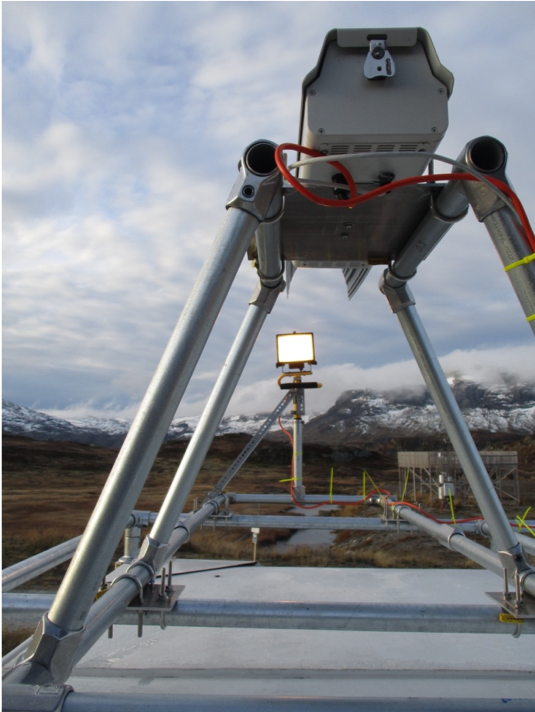
\includegraphics[width=0.35\textwidth]{./fig_instruments/PiP.png}
% 	\caption{PiP}\label{fig:PiP}
% \end{figure}

\begin{wrapfigure}[21]{r}{0.44\textwidth}
	\vspace{-\normalbaselineskip}
	\centering
	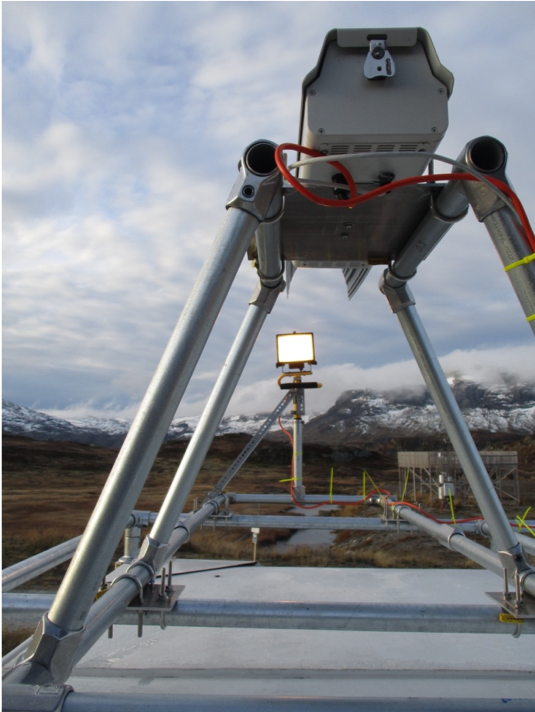
\includegraphics[trim={3.cm, 3.3cm, .5cm, 0cm},clip,width=0.4\textwidth]{./fig_instruments/PiP.png}
	%	\vspace{-10pt}
	\caption{Precipitation Imaging Package at Haukeliseter mounted at the \textbf{container} pointing towards the double fence gauge.}\label{fig:PiP}
	\vspace{-\normalbaselineskip}
\end{wrapfigure}
%%%%%%%%%%%%%%%%%%%%%%%%%%%%%%%%%%%%%%%%%%%%%%%%%%%%%%%%%%%%%%%%%%%%%%%%%%
The precipitation imaging package (PiP) is a modification of the Snowflake Video Imager presented by \cite{newman_presenting_2009}. The video distrometer is a construct of a halogen flood lamp and a video system (\Cref{fig:PiP}). The instrument determines the habit of snowflakes from images at a frequency of \SI{60}{\Hz}. Lamp and lens have a distance of approximately \SI{3}{\metre} which follows a field of view: \SI{32}{\mm} by \SI{24}{\mm}. Hence snowflakes from grey-scale images, particle size distribution (PSD) and fall-speed of precipitation can be determined. 
\\
In front of the halogen lamp is a frosted window, so that the background light is uniform over all time. A falling particle appears as a 2-D shadow in the video image. \cite{newman_presenting_2009} describes in detail the algorithm applied to the system to get information about the snow-particle habit. \\
Winds have almost no effect on the result of the video distrometer \citep{newman_presenting_2009}. \textcolor{red}{They also say, to reduce eventual wind effects, should the distrometer be oriented with regard to storm winds (optical axis perpendicular to mean wind). Was that the case for Haukeliseter (I'm just curious)???}

\newpage
%%%%%%%%%%%%%%%%%%%%%%%%%%%%%%%%%%%%%%%%%%%%%%%%%%%%%%%%%%%%%%%%%%%%%%%%%%
%%%%%%%%%%%%%%%%%%%%%%%%%%%%%%%%%%%%%%%%%%%%%%%%%%%%%%%%%%%%%%%%%%%%%%%%%%
%%%%%%%%% MASC %%%%%%%%%%%%%%
\section{MASC - Multi-Angular Snowfall Camera}
%%% image MASC %%%%%%%%%%%%%%%%%%%%%%%%%%%%%%%%%%%%%
% !TeX spellcheck = en_GB
% \begin{figure}[h!]
% 	\centering
% 	\begin{subfigure}[b]{0.55\textwidth}
% 		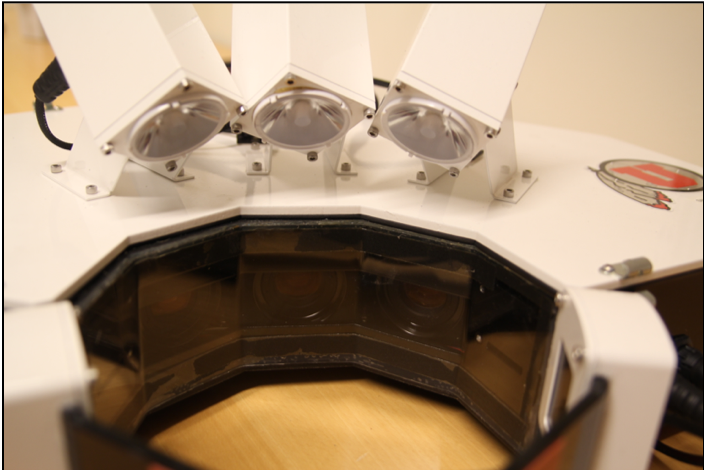
\includegraphics[width=\textwidth]{./fig_instruments/MASC.png}
% 	\end{subfigure}
% 	\begin{subfigure}[b]{0.55\textwidth}
% 		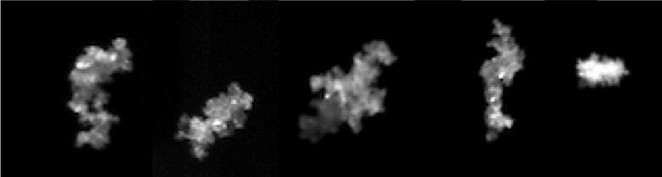
\includegraphics[width=\textwidth]{./fig_instruments/MASC_snowflakes.png}
% 	\end{subfigure}
% 	\caption{Instrument MASC, and images taken by the instrument. \textcolor{red}{lower panel taken from \cite{cooper_variational_2017} maybe we get one for Haukeli?}}\label{fig:MASC}
% \end{figure}

% \begin{wrapfigure}[17]{r}{0.44\textwidth}
\begin{wrapfigure}[15]{r}{0.44\textwidth}
	\vspace{-\normalbaselineskip}
	\centering
	\begin{subfigure}[b]{0.4\textwidth}
		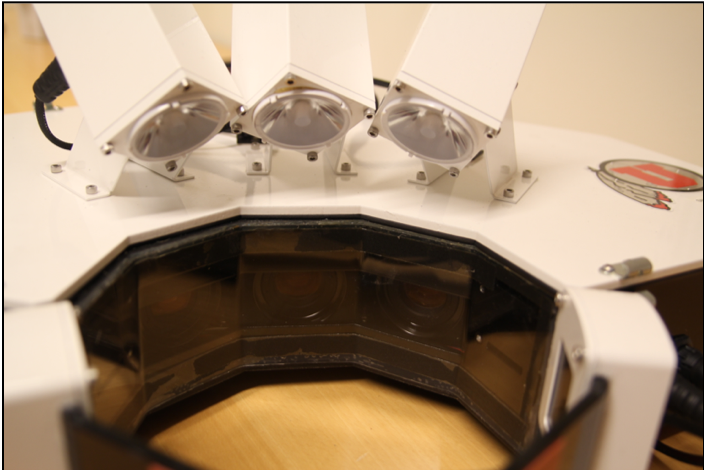
\includegraphics[trim={1.cm, 0cm, .8cm, 0cm},clip,width=\textwidth]{./fig_instruments/MASC.png}
	\end{subfigure}	
	\begin{subfigure}[b]{0.4\textwidth}
		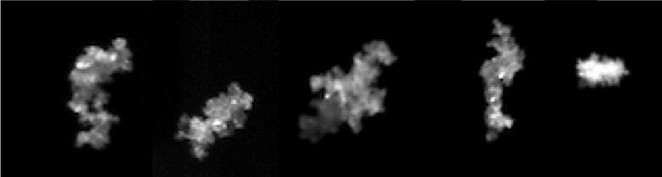
\includegraphics[width=\textwidth]{./fig_instruments/MASC_snowflakes.png}
	\end{subfigure}	
	\caption{Multi-Angular Snowfall Camera and images taken by the instrument during the Christmas storm 2016. Located on \textbf{container}.}\label{fig:MASC}
	%	\vspace{-\normalbaselineskip}
\end{wrapfigure}
%%%%%%%%%%%%%%%%%%%%%%%%%%%%%%%%%%%%%%%%%%%%%%%%%%%%%%%%%%%%%%%%%%%%%%%%%%
Instruments like the afore mentioned PiP has according to \cite{garrett_fall_2012} coarser resolution and the determination of particle size can have size errors. Hence, a new instrument was developed. The Multi-Angular Snowfall Camera (MASC) takes high-resolution images of hydrometeors in free fall and measures the fall-speed simultaneously . \\
The MASC consists of three cameras, three flashes, and two near-infrared sensors, pointing at a ring centre (\Cref{fig:MASC}). A hydrometeor has to pass through the ring in a certain way to trigger the near-infrared sensors. At the same time the three cameras take a picture of the falling particle. Since the cameras take pictures from three different angles, the particles size, shape, and orientation can be specified from the image and an algorithm, described in \cite{garrett_fall_2012}. Furthermore, the heritage of the hydrometeor, such as collision-coalescence, riming , capture nucleation, or aggregation, can be determined as well as the form. \\
The near-infrared sensor, that is used to trigger the cameras and the lights quantifies the fall-speed of the hydrometeors, by measuring the time the particle needs to pass the distance between the upper and lower trigger.    




%%%%%%%%%%%%%%%%%%%%%%%%%%%%%%%%%%%%%%%%%%%%%%%%%%%%%%%%%%%%%%%%%%%%%%%%%%
%%%%%%%%%%%%%%%%%%%%%%%%%%%%%%%%%%%%%%%%%%%%%%%%%%%%%%%%%%%%%%%%%%%%%%%%%%
%%%%%%%%% OPTIMAL ESTIMATION RETRIEVAL %%%%%%%%%%%%%%
\section{Optimal Estimation Retrieval Algorithm} %Section - 1.2
\label{sec:retrieval}
Since 2006, with the launch of CloudSats Cloud Profiling Radar (CPR) a global estimation of snowfall can be done. Several studies, such as \cite{kulie_utilizing_2009} have shown that estimated snowfall values depend heavily upon assumed snowflake microphysical properties.
%\textcolor{red}{Steve had some insertions but no comments.}
%depending on the retrieval assumption, snowfall estimation can give the same values for different a priori guess, e.g. snowflake microphysical properties. 
%Introducing information from snow microphysics will reduce the non-uniqueness in optimal estimation radar retrieval schemes. 
%This can be done by using the temperature at a lower level as a priori as the CloudSat retrieval does.  
%\\
\cite{wood_microphysical_2015} showed that a refinement of the CloudSat snowfall retrieval algorithm can be done by using snowflake models. 
%\textcolor{red}{That was Steves comment which is exactly what I wrote? "
This study was based on data from the Canadian CloudSat-CALIPSO Validation Project \citep[C3VP,][]{hudak_canadian_2006}, where they concentrated on cold season clouds and precipitation.
%"} 
\\
\noindent In an attempt to reduce the non-uniquness of the problem, \cite{wood_microphysical_2015} used the a priori knowledge of snowfall microphysics and temperature (from ground-based observations) to refine the forward-model assumptions for the CloudSat snowfall retrieval scheme. 
%\textcolor{red}{Steve: "They also used a temperature to introduce a priori information on particle size into the retrieval scheme. " Me: They did? So by introducing a temp they estimate the particle size?}
Results from this scheme showed a good agreement with reported values observed at meteorological measurement sites. \\
Model estimates have proven, how useful the estimation retrieval can be to verify ground-based radar snowfall measurements \citep{norin_intercomparison_2015}.
Although the retrieval has obviously been improved the estimation algorithm, can still lead to uncertainties in the retrievals of up to \SIrange{140}{200}{\percent} \citep{wood_estimation_2011}. 
\\
\noindent The snowfall retrieval assumes an exponential particle size distribution (PSD)
\begin{align}
	N(D) = N_{0} exp(-\lambda D).
	\label{eq:PSD}
\end{align} 
$\lambda$ represents here the PSD slope parameter and $N_{0}$ the number density. 
%$D$ is the particle maximum dimension evaluated from the MASC. 
\\
The optimal estimation technique is based on Gaussian statistics. Minimizing the scalar cost function, $\Phi$ for the snowfall properties, $x$ by; 
\begin{equation}
\begin{split}
\Phi(x,y,a) = &(y- F(x))^T \mathbf{S}_y^{-1} (\mathbf{y}-F(\mathbf{x})) \\
&+(x-a)^T \mathbf{S}_{a}^{-1} (x-a)
\end{split} \label{eq:scalar_cost_fct}
\end{equation}
where, $x$, vector of retrieved snowfall properties (slope parameter and number density); $y$, vector of observation (MRR reflectivity) ; $a$, vector of the a priori guess (temperature dependent); $F$, forward model; $\mathbf{S}_a$, a priori error covariance matrix; $\mathbf{S}_y$, measurement error covariance matrix.
\\
\cite{cooper_variational_2017} developed a technique to combine MRR, MASC, and PiP information into a common retrieval framework. Specifically, estimates of snowflake microphysical properties from the MRR are used as the a priori term in the optimal-estimation retrieval scheme. The usage of either MASC\,/\,PiP or MRR fall-speed can show which a priori guess in the retrieval gives the more accurate retrieved snowfall rate at the ground. \\
The difference between the retrieval and the snow gauge observations was \SI{-18}{\percent} when applied to data from Barrow, Alaska.\\
\cite{cooper_variational_2017} also showed that the retrieval is sensitive to habit and fall speed. The installation of a MRR, MASC, and PIP should help to adjust the particle models for graupels and rimed particles which are often observed at Haukeliseter. 

\section{The estimation retrieval step-by-step}
To find a relation between the reflectivity and the preciptiation amount several steps and assumptions have to be done. The following lines, will give a detailed information on the steps, and relate that to \Cref{eq:scalar_cost_fct}. 
\\
\subsection*{Temperature from measurement site}
%%% image surface temperature %%%%%%%%%%%%%%%%%%%%%%%%%%%%%%%%%%%%%
% !TeX spellcheck = en_GB
\begin{figure}[H]
	\centering
	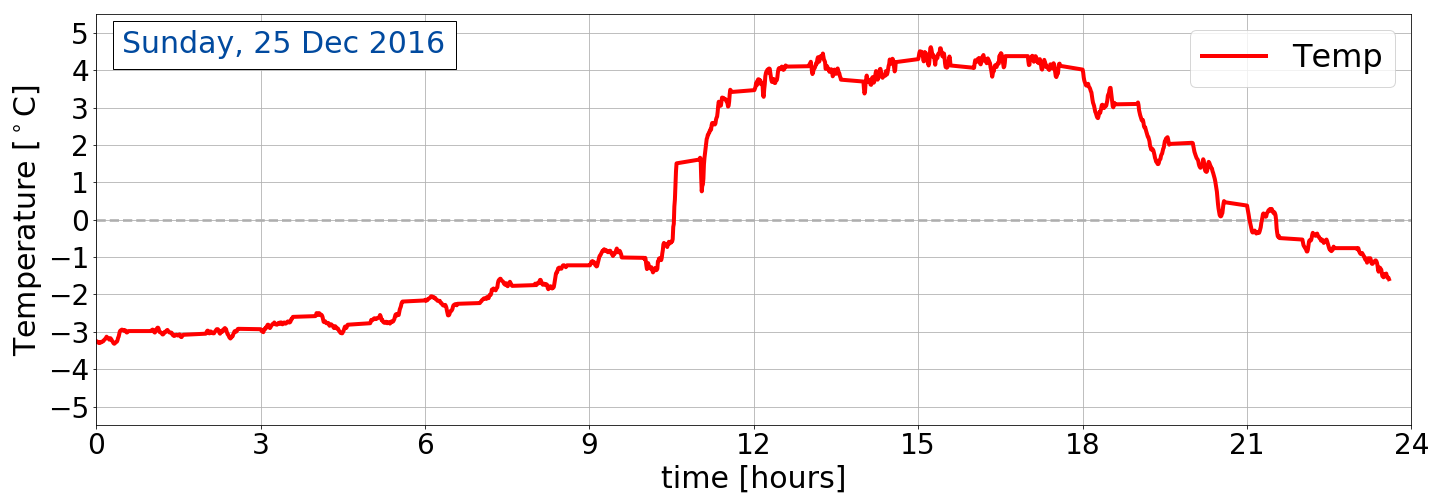
\includegraphics[width=0.6\textwidth]{./fig_weathermast/sfc_temp_20161225}
	\caption{Surface temperature at Haukeliseter every minute, for  \SI{25}{\dec}.}\label{fig:sfc_temp}
\end{figure}
%%%%%%%%%%%%%%%%%%%%%%%%%%%%%%%%%%%%%%%%%%%%%%%%%%%%%%%%%%%%%%%%%%%%%%%%%%
At the Haukeliseter measurement site has in addition a weather mast to full fill the World Meteorological Organization (WMO) requirements. At the weather mast is a temperature sensor, measuring every minute in two meter height. \\
This temperature looks like in \Cref{fig:sfc_temp} and is used as the vector of the a priori guess ($a$) in \Cref{eq:scalar_cost_fct}

\subsection*{MRR measurements}
%%% image surface temperature %%%%%%%%%%%%%%%%%%%%%%%%%%%%%%%%%%%%%
% !TeX spellcheck = en_GB
\begin{figure}[H]
	\centering
	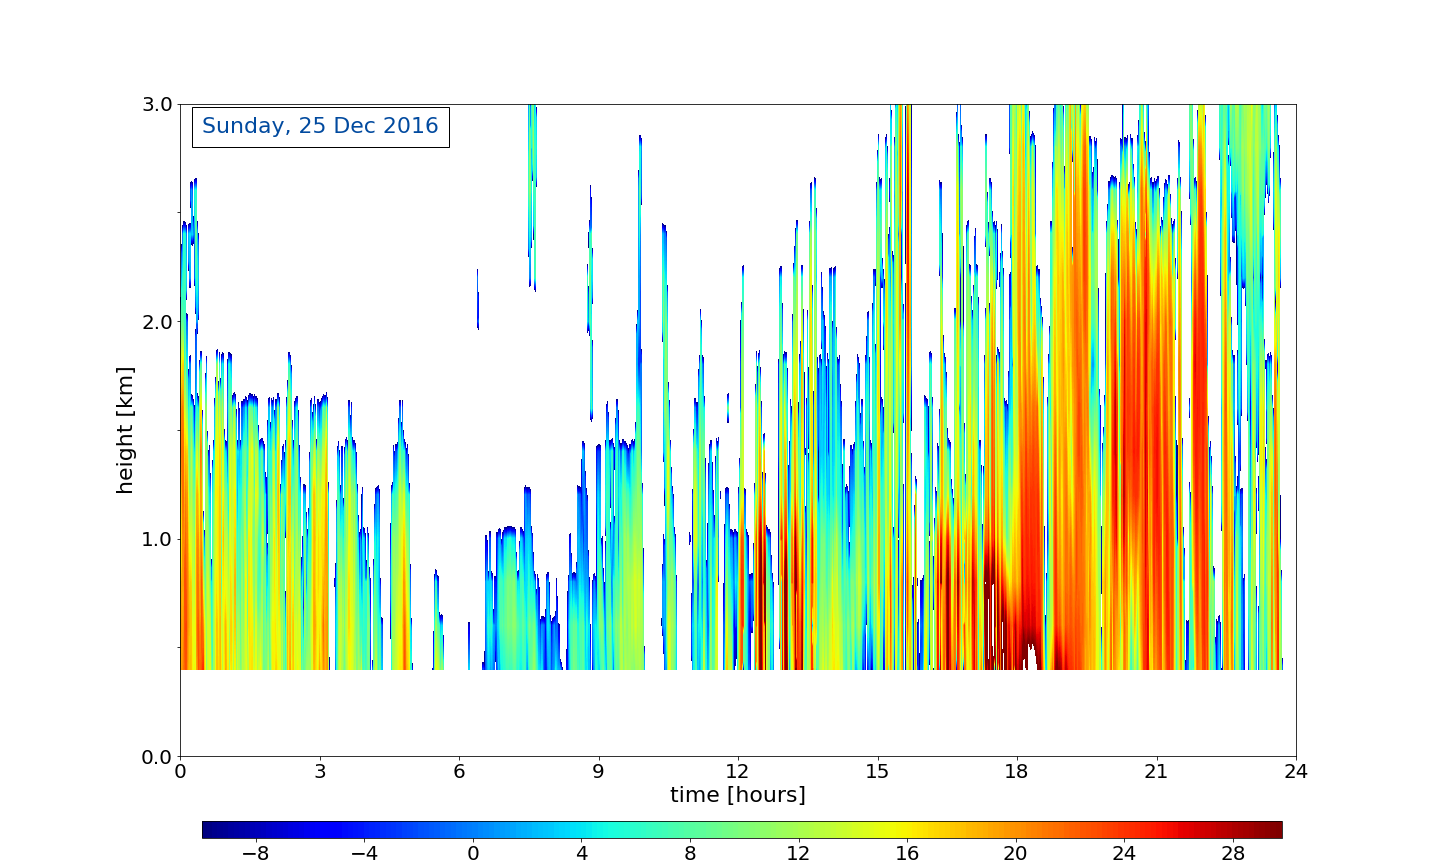
\includegraphics[width=0.6\textwidth]{./fig_MRR/MRR_20161225}
	\caption{Surface temperature at Haukeliseter every minute, for  \SI{25}{\dec}.}\label{fig:MRR_refl}
\end{figure}
%%%%%%%%%%%%%%%%%%%%%%%%%%%%%%%%%%%%%%%%%%%%%%%%%%%%%%%%%%%%%%%%%%%%%%%%%%
Observations from the MRR ($y$) are used in \Cref{eq:scalar_cost_fct}.
Radar reflectivity ($z$) from the MRR is already transformed from \SI{1}{\mm^6\per\metre^3} to \SI{}{\decibel\,Z}.
The transformations is done by the following relationship;
\begin{equation}
Z = 10 \log_{10} \left(\frac{z}{\SI{1}{\mm^6\per\metre^3}}\right) \qquad \text{[\SI{}{\decibel Z}]} 
\end{equation}
Finding a relationship between reflectivity and particle size, common PSD's are used. In the here presented snowfall retrieval an exponential size distribution is assumed (\Cref{eq:PSD}). Attention should be paid, that here snowfall is estimated, where most retrievals use rain. Relationships between reflectivity and snowfall have been developed. Even if the distribution is known, different crystal shapes lead to different results. Furthermore, vary snow density significantly from storm to storm, where small particles are still Rayleigh scattered, and larger particles non-Rayleigh scattered \citep{gunn_microwave_1954}. 
\begin{table}[H]
	\begin{center}
		\caption{Typical reflectivity values, from \cite{} \textcolor{red}{citation here}. }\label{tab:ref_values}
		\begin{tabular}{l|c}
			\hline \hline
			giant hail & \SI{75}{\decibel Z} \\ \hline
			heavy rain & \SI{45}{\decibel Z}\,-\,\SI{50}{\decibel Z} \\ \hline
			heavy snow & \SI{25}{\decibel Z}  \\ \hline
			fog droplets & \SI{-28}{\decibel Z}\\
			\hline
		\end{tabular}
	\end{center}
\end{table}
Only from \Cref{fig:MRR_refl} and \Cref{tab:ref_values} one can not estimate, if snow or rain was present on \SI{25}{\dec}.





\subsection*{Scattering model}
$F$, forward model in \Cref{eq:scalar_cost_fct}.
\subsection*{Final result}
Snowfall retrieval.

% %%% ***************** CHAPTER MEPS ***************** %%%
\chapter{Numerical forecast model}
MEPS was newly operational at Met-Norway when the extreme weather occurred in Norway. Comparing model data with actual observations helps to verify the agreement between model prediction and ground based measurements. 

%%%%%%%%%%%%%%%%%%%%%%%%%%%%%%%%%%%%%%%%%%%%%%%%%%%%%%%%%%%%%%%%%%%%%%%%%%
%%%%%%%%%%%%%%%%%%%%%%%%%%%%%%%%%%%%%%%%%%%%%%%%%%%%%%%%%%%%%%%%%%%%%%%%%%
%%%%%%%%% MEPS %%%%%%%%%%%%%%
\section{AROME - MetCoOP}
\label{sec:MEPS}
AROME-MetCoOp was operational from March 2014 until November 2016, when it was replaced with an ensemble prediction system (EPS) based on AROME-MetCoOp.
MEPS is used as weather forecast at the Norwegian Meteorological Institute, the Swedish Meteorological and Hydrological Institute (SMHI) and the Finnish Meteorological Institute (FMI), \citep{muller_arome-metcoop:_2017, koltzow_metcoop_2017}. 
\\
In principle MEPS is a short-term weather forecast of \SI{66}{\hour} with 10 ensemble member and a horizontal resolution of \SI{2.5}{\km} and 65 vertical levels. In the following section, the model configuration will be briefly explained as well as the motivation for the study case presented.
\\
The orange frame in \Cref{fig:site} shows the MEPS model domain for December 2016. It covers the Nordic Countries including open water such as the Atlantic Ocean, the North and the Baltic Sea.  
\\
The centre of the model is approximately at \ang{63.5}\,N, \ang{15}\,E. 
The horizontal grid points are projected on a Lambert projection to receive same area size of each grid cell. 
The outer, parent grid is the ECMWF-IFS model (European Centre for Medium-Range Weather Forecasts Integrated Forecasting System) with a horizontal resolution of \SI{9}{\km} \citep{homleid_verification_2016}. 
\\
Vertical hybrid coordinates are terrain-following and are mass-based, \citep{muller_arome-metcoop:_2017}. Furthermore, it does underlie non-hydrostatic dynamics, \citep{wiki_description_2017}.
\\
The representation of snow is covered by a modification of the three-class ice parametrization (ICE3) scheme. Where liquid-phase processes are separated from slow ice-phase processes. To model the snow cover an one-layer atmosphere model scheme is implemented. This includes three variables such as: snow water equivalent (SWE), snow density, and snow albedo \citep{muller_arome-metcoop:_2017}.
\\
The MEPS forecasting system consist of 1+9 members where each of the perturbed members perform an initialization of \SI{66}{\hour} at \SIlist{00;06;12;18}{\UTC} \citep{wiki_description_2017}. The ECMWF-IFS forecasts are used \SI{6}{\hour} prior to the actual cycle in MEPS. As synoptic observations are included in the model the snow-depth predictions underlay a special performance. Observations of snow-depth are only available at \SIlist{06;18}{\UTC}, therefore is the snow analysis only performed twice daily \citep{muller_arome-metcoop:_2017, homleid_verification_2016}. 
\\
For more detailed information to the model the reader is referred to \cite{muller_arome-metcoop:_2017} and \cite{wiki_description_2017} and its references therein.

%%%%%%%%%%%%%%%%%%%%%%%%%%%%%%%%%%%%%%%%%%%%%%%%%%%%%%%%%%%%%%%%%%%%%%%%%%
%%%%%%%%%%%%%%%%%%%%%%%%%%%%%%%%%%%%%%%%%%%%%%%%%%%%%%%%%%%%%%%%%%%%%%%%%%
%%%%%%%%% MEPS %%%%%%%%%%%%%%
\section{MEPS Data processing}
\label{sec:MEPS_process}
To compare the measurements from the surface with the MEPS data, the colsest grid point is used to Haukeliseter.
\\
MEPS has a vertical resolution in hybrid sigma pressure coordinates (0-1). The zero sigma level is at the top of the atmosphere, hence positive values are downward. To calculate the actual vertical pressure in \SI{}{\Pa}, a formula is provided in the OPeNDAP Dataset of \texttt{meps\_full\_2\_5km\_*.nc} by \cite{norwegian_meteorological_institute_met_2016}.  
\begin{align}
	p(n,k,j,i) = ap(k) + b(k) \cdot ps(n,j,i) \qquad [\SI{}{\Pa}].
	\label{eq:hybrid_sigma_pressure}
\end{align}
$ps$ is the surface air pressure in \SI{}{\Pa}, and information about the variables $ap$, $b$ are not given from the access form. \textcolor{red}{Maybe check in the documentation from BJ?!}  
\\
The next step was to convert pressure-levels into actual heights by the use of the hypsometric equation. Here, the air temperature in model levels is used to calculate the mean temperature of each layer. 
\begin{align}
	\overline{T} = \dfrac{\int\limits_{p2}^{p1} T \partial ln p}{\int\limits_{p2}^{p1}\partial ln p} \qquad [\SI{}{\kelvin}]
	\label{eq:T_avg}
\end{align}
For the numerical integration, the Simpson rule was used, which is a build-in function in Python. \\
In the book from \cite{martin_mid-latitude_2006} steps of differentiating the hypsometric equation are presented by using the virtual temperature. But when the atmospheric mixing ratio is large, will the virtual temperature only be \SI{1}{\percent} larger than the actual air temperature. 
\\
The thickness, $\Delta z$, of each layer is then be found by using the hypsometric equation from \cite{martin_mid-latitude_2006} and the previously calculated mean temperature (\Cref{eq:T_avg}):
\begin{equation}
\begin{split}
\Delta z & = z_2 - z_1 \\
& = \frac{R_d \overline{T}}{g} ln(\frac{p_1}{p_2}), \qquad [\SI{}{\metre}]
\end{split}
\label{eq:hypsometric}
\end{equation}
where $R_d$ is gas constant for dry air with a value of \SI{287}{\joule\per\kilogram\per\kelvin},  standard gravity $g\,=\,$\SI{9.81}{\metre\per\square\second}. $p_1$ and $p_2$ are the pressure levels at lower and higher levels, respectively ($p_2 < p_1$).


